%contient des exemples d'homographies traité par nous et ripmap

\sse{Visual comparison between the Ripmap and the new geometric decomposition}
%\sse{Comparaison du Ripmap et de la décomposition géométrique}

The previous part presented numerical results without showing where, on a given resampling, the geometric decomposition is better than the Ripmap. This part focuses on comparing the Ripmap and the geometric decomposition for different homographies (figures \ref{Homo1}, \ref{Homo2}, \ref{Homo3}, \ref{Homo4}, \ref{Homo5} and \ref{Homo5det}) to highlight where the geometric decomposition presents can be better than the Ripmap. Each time, the same homography is used to resample the same image using different methods.
%Cette section décrit succintement les expériences représentées aux figures \ref{Homo1}, \ref{Homo2}, \ref{Homo3}, \ref{Homo4}, \ref{Homo5} et \ref{Homo5det}. On a choisit des homographies éloignées des cas dégénérés.


One can notice that the geometric decompostion can reduce aliasing (figures \ref{Homo1}, \ref{Homo4} and \ref{Homo5}). For homographies squeezing the image in a diagonal direction, the geometric decomposition reduces the blur (figure \ref{Homo2}). Nevertheless for some homographies both methods give similar results (figure \ref{Homo3}).


%On peut remarquer que la décomposition permet pour certaines homographies de limiter l'\emph{aliasing} (Homographies 1, 4 et 5). Dans le cas d'une déformation en diagonale elle limite le flou (Homographie 2). Il existe néanmoins des cas où les deux méthodes ont des performances comparables (Homographie 3).

The execution time of the program was of about one second for an image of size $512\times 512$ on a dual-core laptop computer.

%Le programme a un temps d'éxecution de l'ordre d'une seconde sur une image $512\times 512$ avec un laptop à deux processeurs.

\begin{figure}
\subfigure[Geometric decomposition]{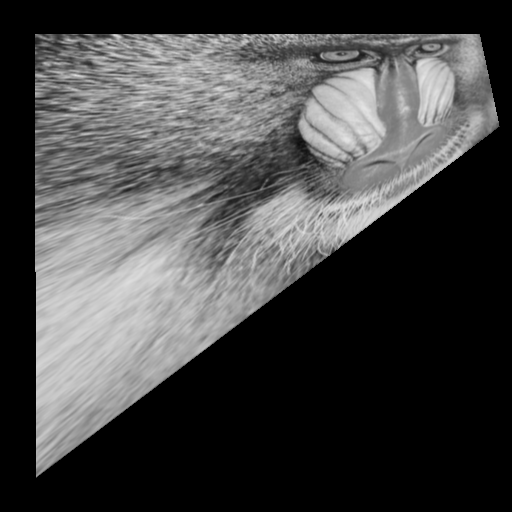
\includegraphics[scale=0.4]{img_f_1.png}}
\subfigure[Ripmap]{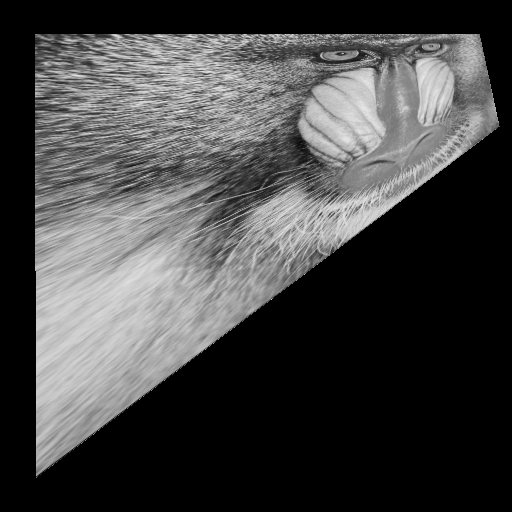
\includegraphics[scale=0.4]{img_ripmap_1.png}}
\caption{The geometric decomposition method creates less aliasing}
\label{Homo1}
\end{figure}

%\begin{figure}
%\subfigure[Décomposition géométrique]{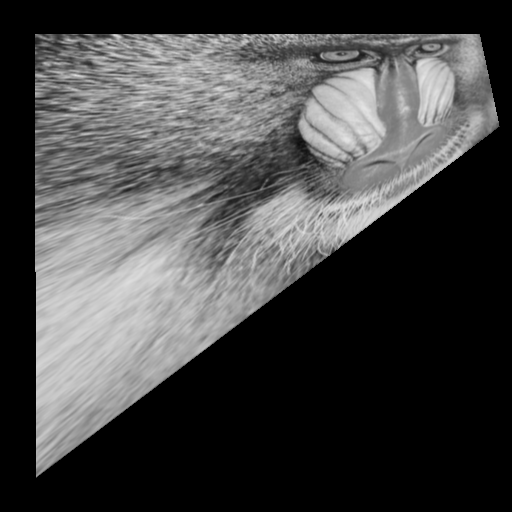
\includegraphics[scale=0.4]{img_f_1.png}}
%\subfigure[Ripmap]{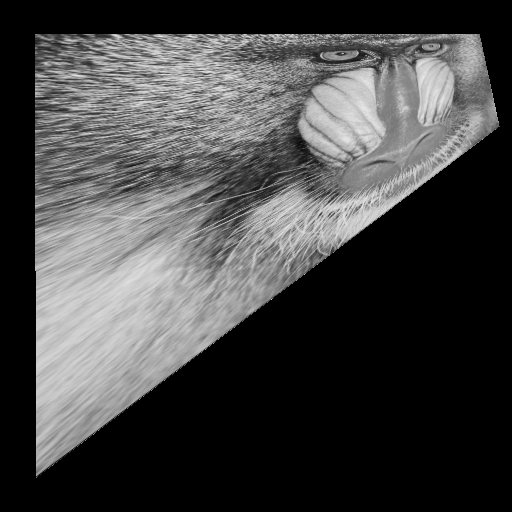
\includegraphics[scale=0.4]{img_ripmap_1.png}}
%\caption{Homographie 1 : La décomposition géométrique produit moins d'\emph{aliasing}}
%\label{Homo1}
%\end{figure}

\begin{figure}
\subfigure[Geometric decomposition]{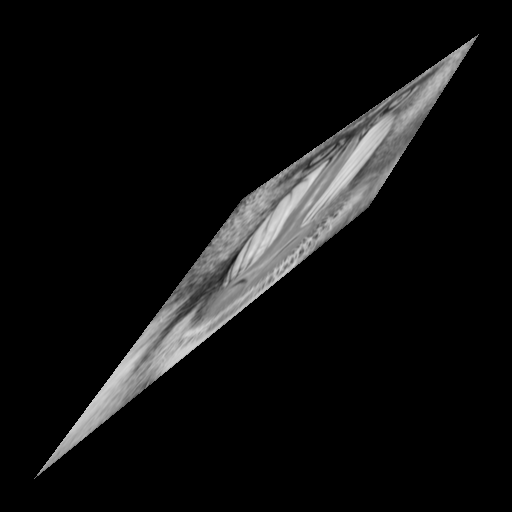
\includegraphics[scale=0.4]{img_f_2.png}}
\subfigure[Ripmap]{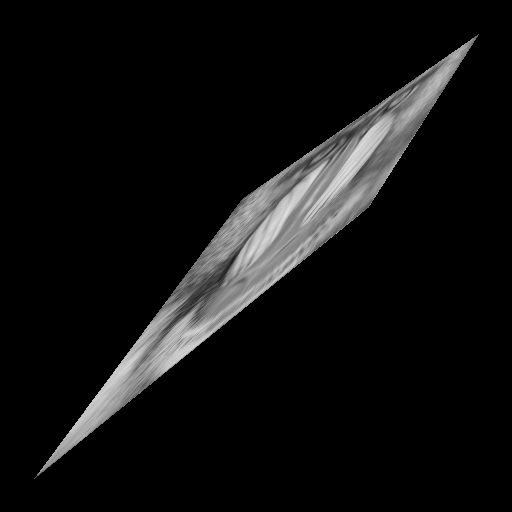
\includegraphics[scale=0.4]{img_ripmap_2.png}}
\caption{The geometric decomposition method does not create excessive blur (see section \ref{Ripmap}).}
\label{Homo2}
\end{figure}



%\begin{figure}
%\subfigure[Décomposition géométrique]{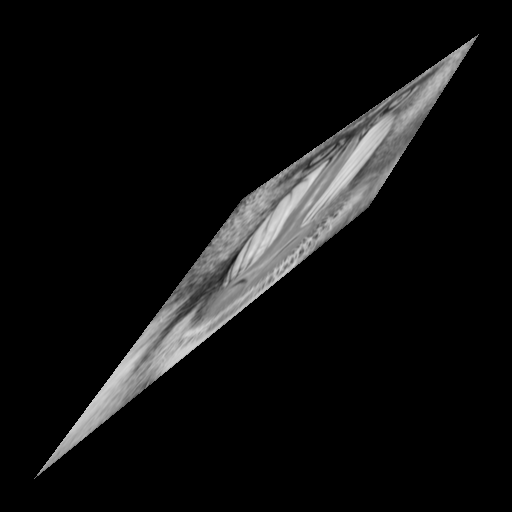
\includegraphics[scale=0.4]{img_f_2.png}}
%\subfigure[Ripmap]{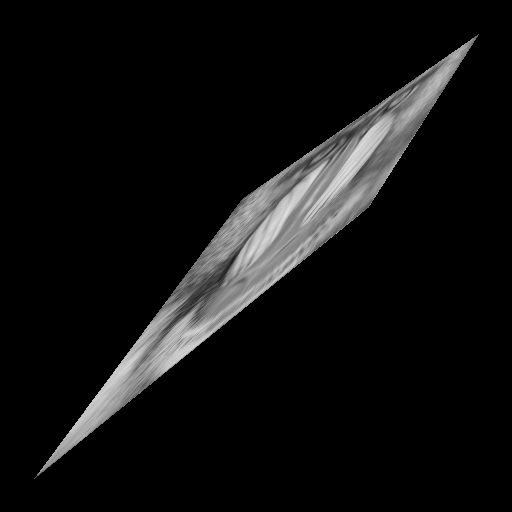
\includegraphics[scale=0.4]{img_ripmap_2.png}}
%\caption{Homographie 2 : La décomposition n'entraine pas d'\emph{over-blurring} (voir section \ref{Ripmap})}
%\label{Homo2}
%\end{figure}


\begin{figure}
\subfigure[Geometric decomposition]{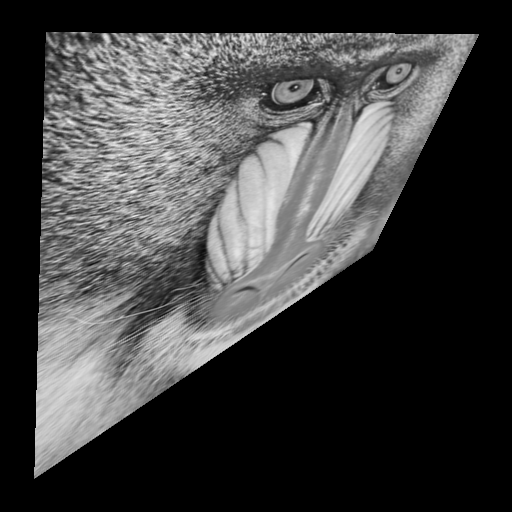
\includegraphics[scale=0.4]{img_f_3.png}}
\subfigure[Ripmap]{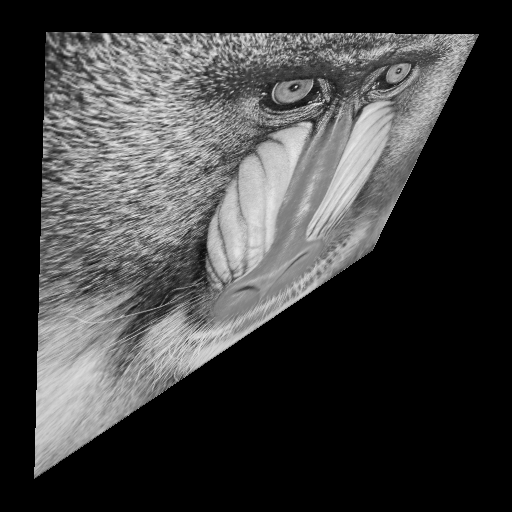
\includegraphics[scale=0.4]{img_ripmap_3.png}}
\caption{None of the methods seems to clearly prevail, still the decomposition introduced a bit less aliasing.}
\label{Homo3}
\end{figure}


%\begin{figure}
%\subfigure[Décomposition géométrique]{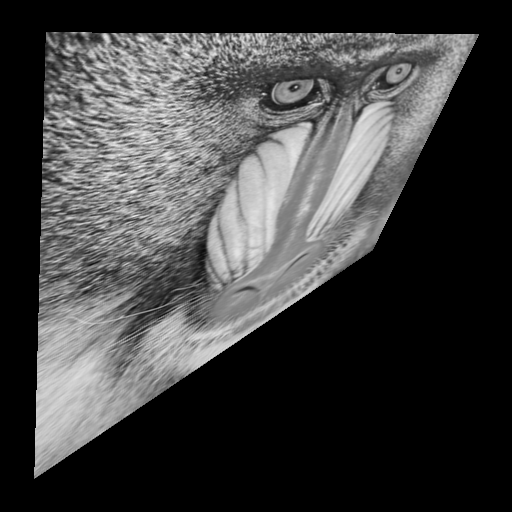
\includegraphics[scale=0.4]{img_f_3.png}}
%\subfigure[Ripmap]{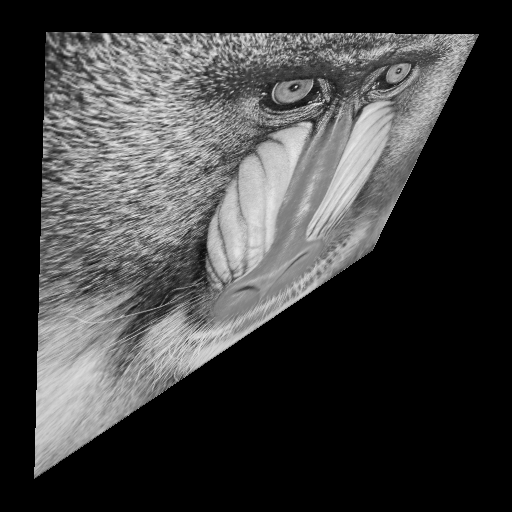
\includegraphics[scale=0.4]{img_ripmap_3.png}}
%\caption{Homographie 3 : Aucune des deux méthodes n'est clairement meilleure}
%\label{Homo3}
%\end{figure}

\begin{figure}
\subfigure[Geometric decomposition]{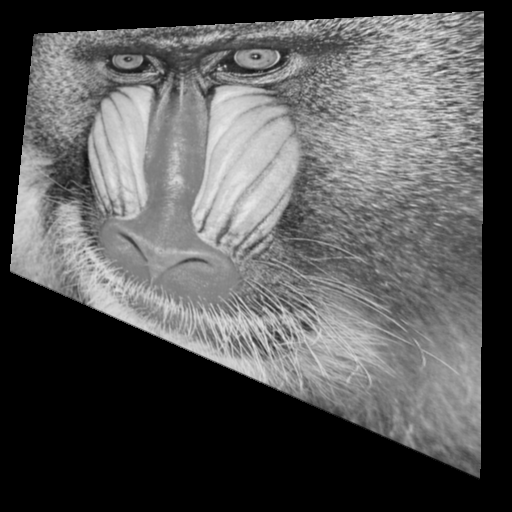
\includegraphics[scale=0.4]{img_f_4.png}}
\subfigure[Ripmap]{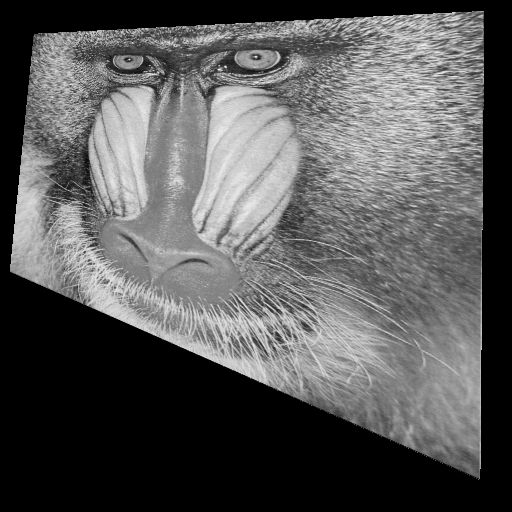
\includegraphics[scale=0.4]{img_ripmap_4.png}}
\caption{ The geometric decomposition method creates less aliasing.}
\label{Homo4}
\end{figure}

%\begin{figure}
%\subfigure[Décomposition géométrique]{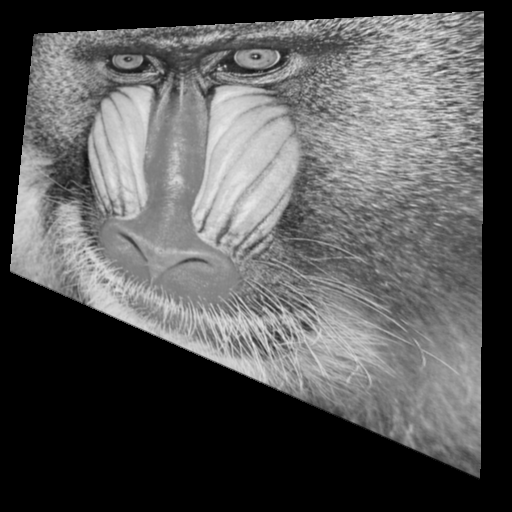
\includegraphics[scale=0.4]{img_f_4.png}}
%\subfigure[Ripmap]{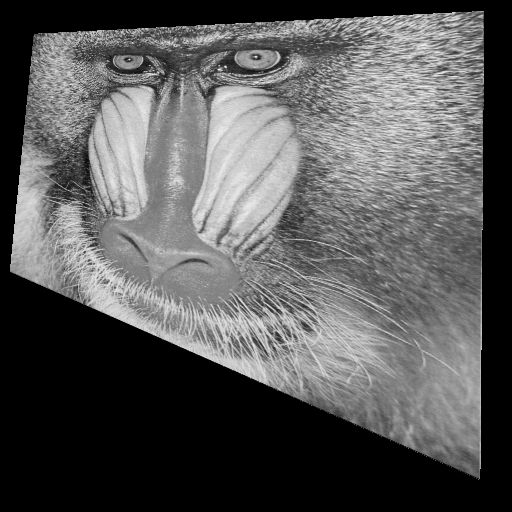
\includegraphics[scale=0.4]{img_ripmap_4.png}}
%\caption{Homographie 4 : La décomposition géométrique produit moins d'\emph{aliasing}}
%\label{Homo4}
%\end{figure}



\begin{figure}
\subfigure[Geometric decomposition]{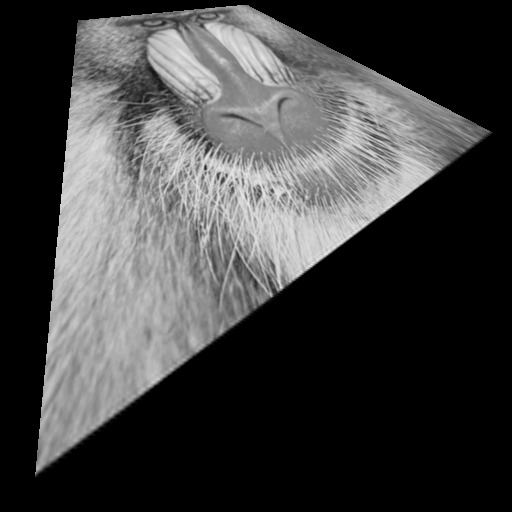
\includegraphics[scale=0.4]{img_geo_5.png}}
\subfigure[Ripmap]{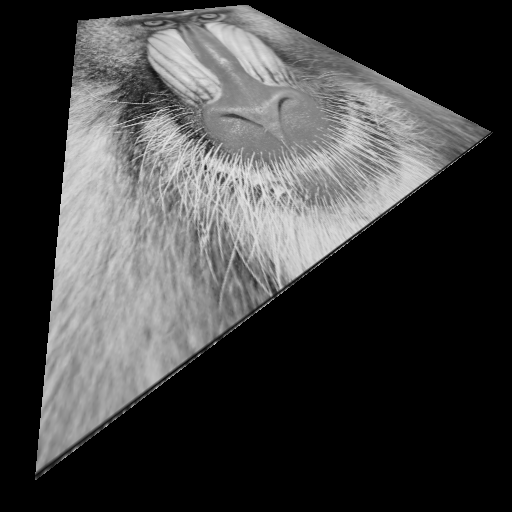
\includegraphics[scale=0.4]{img_ripmap_5.png}}
\subfigure[Naive method]{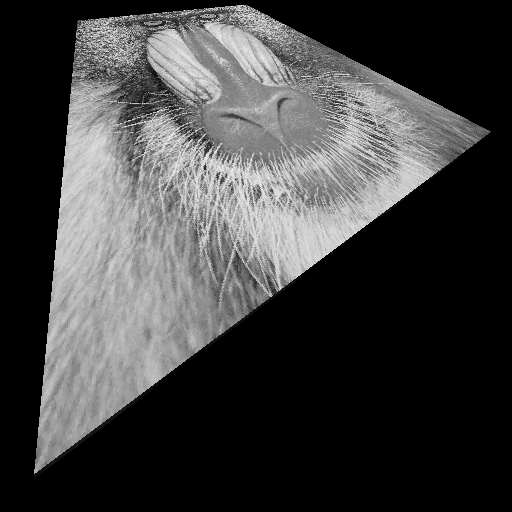
\includegraphics[scale=0.4]{img_naive_5.png}}
\subfigure[Mipmap]{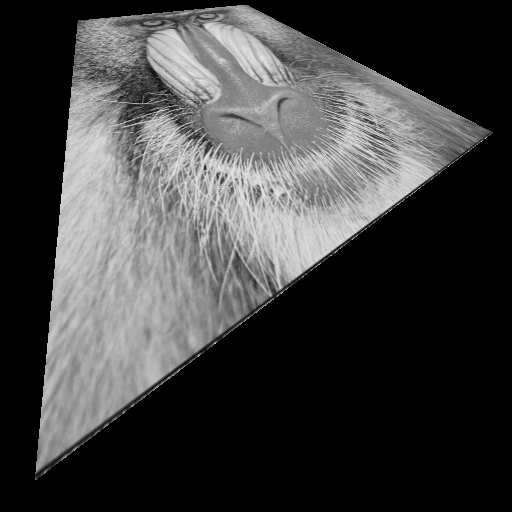
\includegraphics[scale=0.4]{img_mipmap_5.png}}
\caption{The geometric decomposition method creates less aliasing. See the detail on figure \ref{Homo5det}.}
\label{Homo5}
\end{figure}

%\begin{figure}
%\subfigure[Décomposition géométrique]{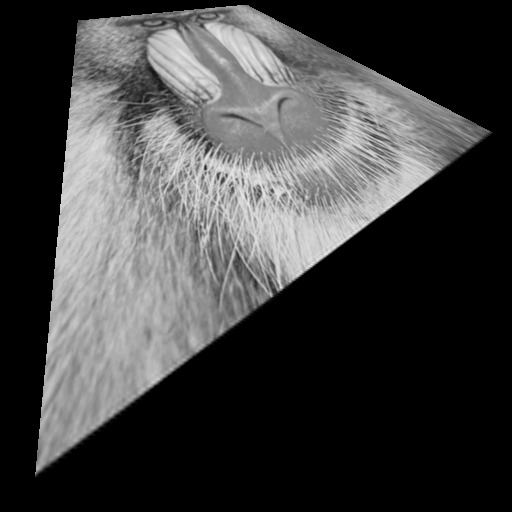
\includegraphics[scale=0.4]{img_geo_5.png}}
%\subfigure[Ripmap]{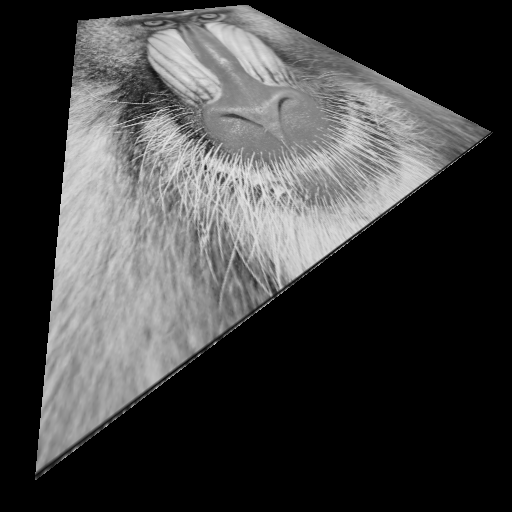
\includegraphics[scale=0.4]{img_ripmap_5.png}}
%\subfigure[Méthode naive]{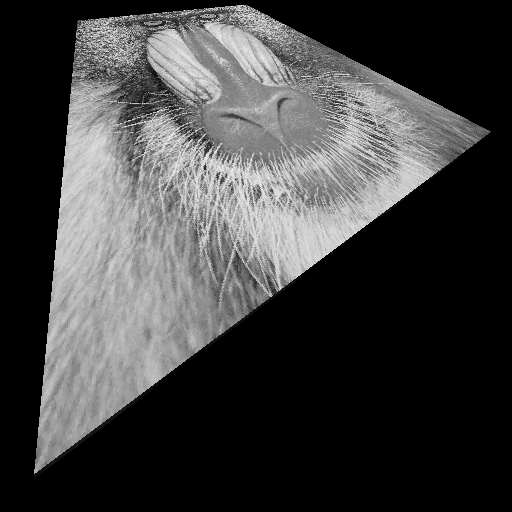
\includegraphics[scale=0.4]{img_naive_5.png}}
%\subfigure[Mipmap]{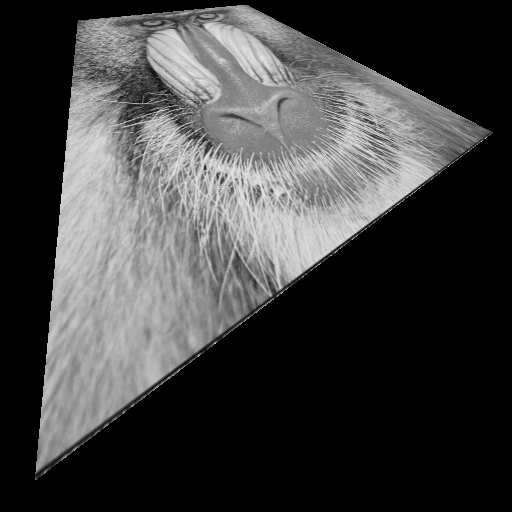
\includegraphics[scale=0.4]{img_mipmap_5.png}}
%\caption{Homographie 5 : La décomposition produit moins d'aliasing, un détail est présenté dans la figure \ref{Homo5det}}
%\label{Homo5}
%\end{figure}


\begin{figure}[t]
\centering
\subfigure[Naive method]{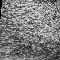
\includegraphics[scale=1.25]{img_det_naive.png}}\hfill
\subfigure[Mipmap]{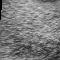
\includegraphics[scale=1.25]{img_det_mipmap.png}}\hfill
\subfigure[Ripmap]{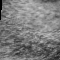
\includegraphics[scale=1.25]{img_det_ripmap.png}}\hfill
\subfigure[Geometric decomposition]{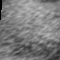
\includegraphics[scale=1.25]{img_det_geo.png}}
\caption{Detail from figure \ref{Homo5} }
\label{Homo5det}
\end{figure}



%\begin{figure}[t]
%\centering
%\subfigure[Méthode naive]{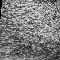
\includegraphics[scale=1.25]{img_det_naive.png}}\hfill
%\subfigure[Mipmap]{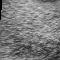
\includegraphics[scale=1.25]{img_det_mipmap.png}}\hfill
%\subfigure[Ripmap]{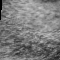
\includegraphics[scale=1.25]{img_det_ripmap.png}}\hfill
%\subfigure[Décomposition géométrique]{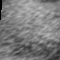
\includegraphics[scale=1.25]{img_det_geo.png}}
%\caption{Détail de l'homographie 5 qui a été présentée dans la figure \ref{Homo5} }
%\label{Homo5det}
%\end{figure}
